\chapter{Introduction}
\section{Motivation}

\section{Objectives}

\chapter{Fundamentals}
\section{ROS}
\section{MCA}
\section{Kinect}
\section{Laser Scanner}
3D laser scanner use narrow laser-beam to scan their environment and allow almost continuous scanning - regardless of whether objects are moving or not. As a result, 3D laser scanner gets a set of points which represent the direction and distance of objects in around. Sick LMS100 (shown in Figure \ref{Laser}) has the scanning angle of  270$^\circ$ and has high detection capability.

We can get the output from laser scanner in ROS with sensor\_masgs/LaserScan message. The message is made up of several parts, including header, ranges, and other information of laser scaner. The start and end angle of the scan, angular distance between measurements, time between measurements, minimum and minimum range value are stored in this message. Most important information we need is the angle of each hit and its distance (range) from the scanner.

\begin{figure}[thpb]
      \centering
      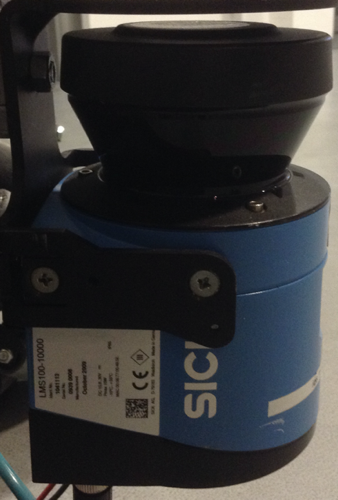
\includegraphics[width=0.5\textwidth]{Laserscanner.png}
      %\includegraphics[scale=1.0]{figurefile}
      \caption{Sick LMS100}
      \label{Laser}
   \end{figure}
\section{ASAP (Advanced Shared Autonomy Platform)}
The ASAP (shown in Figure \ref{ASAP}), short for Advanced Shared Autonomy Platform, is a mobile robotic platform based on two Segway RMP-50 Omni platforms. The Platform is mounted with four omnidirectional plastic rollers, so that the Segway can free move in all directions (shown in Figure \ref{Omni}). In addition, this ASAP includes some sensors, on-board comoputer, software system. For sensor, there are Two Sick LMS100 laser scanners and a Kinect on top. The embeded computer is Esperia, which has 4G ram, 64G SSD, core i7 M620 CPU and can be connected through WLAN address 141.21.13.215. Ubuntu 14.04 Trusty, ROS Indigo, MCA2 are three main software systems in this ASAP.

\begin{figure}[thpb]
      \centering
      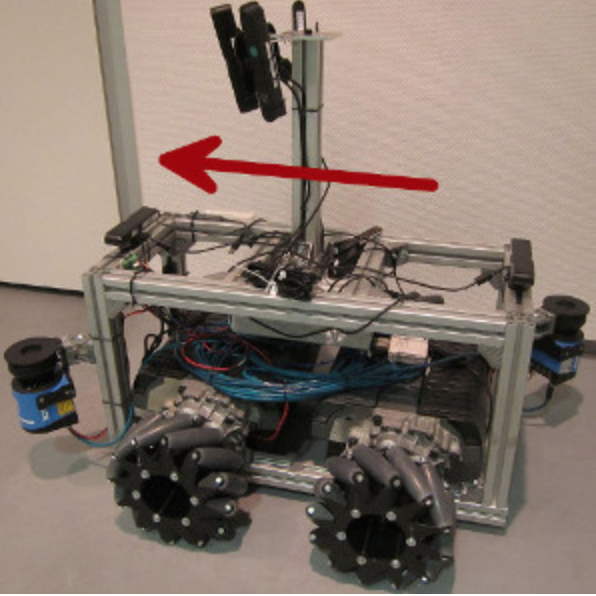
\includegraphics[width=0.5\textwidth]{ASAP.png}
      %\includegraphics[scale=1.0]{figurefile}
      \caption{The structer of Advanced Shared Autonomy Platform, and red arrow shows the forward direction of the platform, which is the same as the X axes in ROS.}
      \label{ASAP}
   \end{figure}

\begin{figure}[thpb]
      \centering
      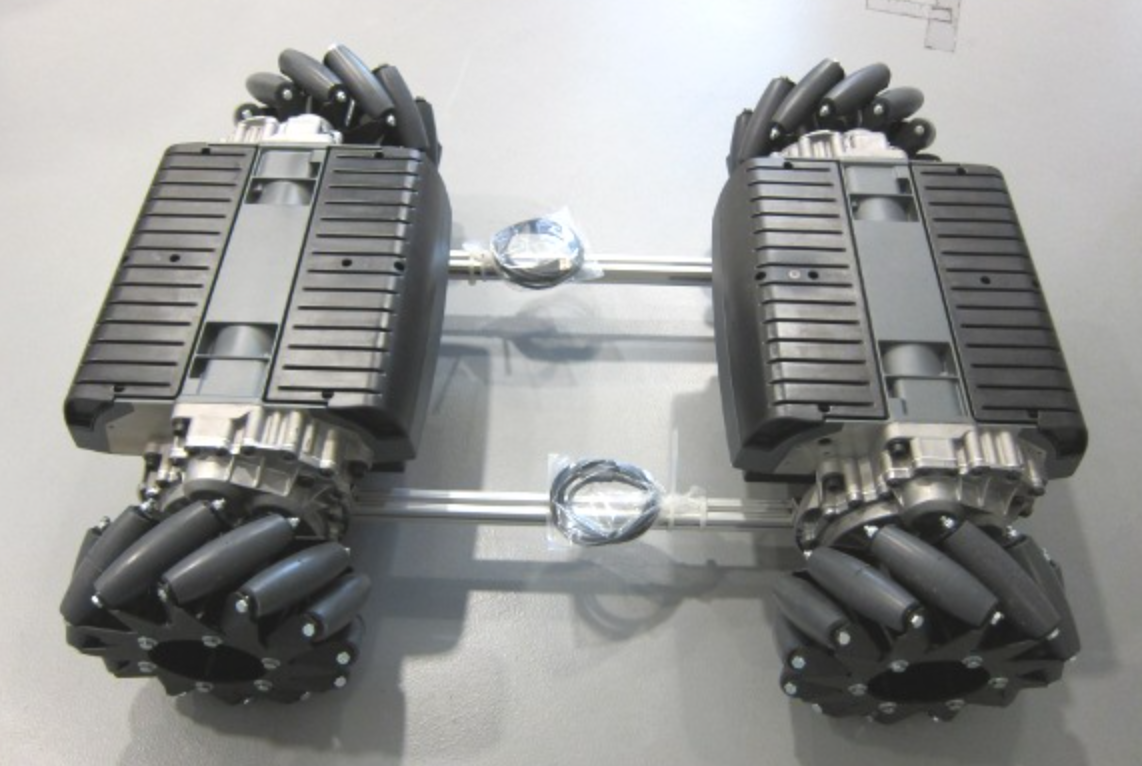
\includegraphics[width=0.5\textwidth]{SegwayPlattform.png}
      %\includegraphics[scale=1.0]{figurefile}
      \caption{The Segway RMP-50 Omni Plattform includes Mecanum-Rad and Batterie.}
      \label{Omni}
   \end{figure}